\chapter{Pola Desain Perilaku 1}


\section{Interpreter}

\subsection{Tujuan dan Konteks Penggunaan}

Pola \textit{Interpreter} adalah pola desain perilaku yang digunakan untuk mendefinisikan representasi gramatika bahasa dan menyediakan cara untuk menginterpretasikan kalimat dalam bahasa tersebut. Pola ini sangat berguna dalam sistem yang memerlukan parsing dan evaluasi terhadap struktur ekspresi berulang, seperti ekspresi matematika, kueri sederhana, atau bahasa domain khusus (DSL - Domain Specific Language).

Tujuan utama dari pola Interpreter adalah untuk:
\begin{itemize}
	\item Mendefinisikan tata bahasa (grammar) dan representasi internal dari suatu bahasa atau ekspresi.
	\item Memberikan antarmuka interpretasi (evaluation) terhadap ekspresi tersebut.
	\item Memisahkan logika interpretasi dari struktur data, dengan pendekatan rekursif berbasis pohon.
\end{itemize}

Struktur pola Interpreter biasanya terdiri dari:
\begin{itemize}
	\item \textbf{AbstractExpression:} Antarmuka atau kelas abstrak yang mendefinisikan metode interpretasi.
	\item \textbf{TerminalExpression:} Mewakili simbol terminal dalam grammar, seperti angka atau variabel.
	\item \textbf{NonTerminalExpression:} Mewakili ekspresi yang terdiri dari satu atau lebih ekspresi lainnya (misalnya ekspresi aritmatika).
	\item \textbf{Context:} Menyimpan informasi global atau lingkungan yang dibutuhkan saat interpretasi.
\end{itemize}

Pola ini cocok digunakan ketika:
\begin{itemize}
	\item Struktur grammar sederhana dan stabil.
	\item Sistem membutuhkan kemampuan interpretasi langsung terhadap input teks atau struktur ekspresi.
	\item Ingin menyediakan antarmuka evaluasi untuk ekspresi berbasis pohon.
\end{itemize}

Beberapa domain aplikasi umum untuk pola Interpreter antara lain:
\begin{itemize}
	\item Mesin ekspresi aritmatika sederhana (calculator).
	\item Sistem pencarian berbasis ekspresi logika (\texttt{AND}, \texttt{OR}, \texttt{NOT}).
	\item Evaluasi query terhadap data (misalnya query mini terhadap koleksi objek).
	\item Penerapan bahasa skrip atau DSL sederhana.
\end{itemize}

Pola ini memperjelas struktur grammar dan membuat implementasi interpreter modular dan mudah diperluas. Namun, pola ini kurang cocok untuk grammar kompleks karena dapat menghasilkan hirarki kelas yang sangat dalam dan sulit dipelihara.


\subsection{Contoh Kasus Penggunaan}

Pola \textit{Interpreter} digunakan secara luas dalam berbagai skenario yang melibatkan evaluasi ekspresi, pemrosesan aturan, atau interpretasi struktur bahasa mini. Penggunaannya sangat sesuai ketika terdapat kebutuhan untuk mengekspresikan aturan dalam bentuk sintaks yang dapat dievaluasi secara fleksibel dan berulang. Berikut adalah beberapa contoh konkret:

\textbf{1. Mesin Ekspresi Aritmatika Sederhana} \\
Salah satu contoh paling umum adalah kalkulator ekspresi aritmatika. Misalnya, ekspresi seperti \texttt{(5 + 3) - 2} dapat direpresentasikan sebagai pohon ekspresi, dan setiap node dalam pohon tersebut diinterpretasikan secara rekursif menggunakan pola Interpreter.

\textbf{2. Pencarian dan Penyaringan Data (Query Filter)} \\
Dalam sistem penyaringan atau pencarian data, pola Interpreter dapat digunakan untuk mengekspresikan kondisi pencarian seperti \texttt{name = 'Alice' AND age > 25}. Setiap kondisi menjadi ekspresi terminal, sedangkan operator logika seperti \texttt{AND}, \texttt{OR}, dan \texttt{NOT} diwakili oleh ekspresi non-terminal.

\textbf{3. Evaluasi Bahasa Domain Khusus (DSL)} \\
Dalam pengembangan DSL (Domain Specific Language), pola Interpreter digunakan untuk memetakan sintaks domain ke dalam struktur evaluasi. Contohnya adalah sistem konfigurasi, alur kerja, atau aturan bisnis seperti \texttt{IF order.total > 500 THEN apply\_discount}.

\textbf{4. Sistem Validasi dan Aturan (Rules Engine)} \\
Sistem yang menerapkan serangkaian aturan atau kebijakan (misalnya, sistem asuransi atau kredit) dapat menggunakan pola Interpreter untuk mengevaluasi aturan berdasarkan data klien. Setiap aturan atau kondisi dapat direpresentasikan sebagai ekspresi yang dapat diinterpretasikan terhadap konteks data.

\textbf{5. Pemrosesan Ekspresi Boolean dalam Game atau AI} \\
Dalam pengembangan game, AI sering memerlukan sistem evaluasi kondisi berbasis logika, misalnya: \texttt{EnemyInRange AND HasAmmo}. Ekspresi ini dapat dibangun dan dievaluasi menggunakan pola Interpreter untuk menentukan keputusan AI.

\textbf{6. Parsing dan Evaluasi Format Bahasa Ringan} \\
Misalnya, evaluasi ekspresi dalam format seperti postfix, prefix, atau ekspresi bahasa konfigurasi seperti JSONPath atau XPath sederhana dapat dibangun menggunakan pola Interpreter, di mana struktur pohon ekspresi dibangun dan diinterpretasikan terhadap data.

Dengan contoh-contoh di atas, pola \textit{Interpreter} terbukti bermanfaat di berbagai bidang mulai dari sistem sederhana hingga sistem evaluasi logika kompleks. Namun, pola ini lebih efektif untuk grammar yang tidak terlalu rumit dan ukuran ekspresi yang tidak terlalu besar.


\subsection{Kelebihan dan Kekurangan}

Pola \textit{Interpreter} menawarkan sejumlah keunggulan dalam hal fleksibilitas dan ekspresivitas dalam merepresentasikan dan mengeksekusi aturan atau ekspresi dalam suatu domain spesifik. Namun, penggunaannya juga memiliki batasan tertentu, terutama dalam hal efisiensi dan skalabilitas.

\textbf{Kelebihan:}
\begin{itemize}
	\item \textbf{Mudah dikembangkan dan diperluas:} Setiap aturan atau ekspresi direpresentasikan sebagai kelas terpisah, sehingga penambahan ekspresi baru cukup dengan menambahkan kelas baru tanpa mengubah struktur yang ada.
	
	\item \textbf{Cocok untuk bahasa domain kecil:} Sangat sesuai digunakan untuk DSL (Domain Specific Language) yang sederhana dan memiliki aturan tetap, seperti bahasa konfigurasi, ekspresi aritmatika, atau aturan logika.
	
	\item \textbf{Struktur ekspresi modular dan komposabel:} Ekspresi dapat dibentuk dari komposisi ekspresi yang lebih kecil secara hierarkis (misalnya pohon ekspresi), memungkinkan evaluasi rekursif yang seragam.
	
	\item \textbf{Memisahkan logika dari data:} Evaluasi ekspresi dapat dilakukan secara terpisah dari struktur data yang mendasari, mendukung prinsip pemisahan tanggung jawab.
	
	\item \textbf{Mudah diimplementasikan dan di-debug:} Untuk grammar kecil, struktur interpretasi sangat eksplisit dan dapat dengan mudah ditelusuri secara manual, sangat berguna dalam sistem edukatif atau prototipe awal.
\end{itemize}

\textbf{Kekurangan:}
\begin{itemize}
	\item \textbf{Kurang efisien untuk grammar besar:} Jika bahasa atau grammar yang ingin ditangani cukup kompleks dan ekspresi sangat banyak, struktur berbasis objek dapat menyebabkan overhead performa dan konsumsi memori yang tinggi.
	
	\item \textbf{Proliferasi kelas:} Setiap simbol atau ekspresi memerlukan satu kelas, sehingga implementasi grammar besar akan menghasilkan banyak kelas kecil yang sulit dikelola.
	
	\item \textbf{Tidak cocok untuk runtime dinamis:} Pola ini lebih cocok untuk grammar statis. Jika aturan berubah-ubah saat runtime, sistem interpreter akan menjadi kurang fleksibel dibanding pendekatan berbasis parser atau rule engine dinamis.
	
	\item \textbf{Debugging dan tracing menjadi kompleks:} Pada struktur ekspresi yang dalam atau rekursif, proses debugging bisa sulit karena alur evaluasi tersebar di banyak objek.
	
	\item \textbf{Sulit dioptimasi secara global:} Karena setiap ekspresi berdiri sendiri dan dievaluasi secara lokal, sulit untuk menerapkan optimisasi menyeluruh seperti memoization atau kompilasi ekspresi.
\end{itemize}

Secara keseluruhan, pola \textit{Interpreter} sangat efektif untuk membangun evaluator bahasa kecil atau aturan terstruktur yang dapat diwakili sebagai ekspresi. Namun, untuk grammar yang lebih besar atau sistem dengan kebutuhan performa tinggi, pendekatan lain seperti parser generator, visitor pattern, atau expression evaluator berbasis AST (Abstract Syntax Tree) mungkin lebih tepat.


\subsection{Implementasi dalam Java}

Implementasi pola \textit{Interpreter} dalam Java umumnya melibatkan pembuatan kelas abstrak atau antarmuka untuk ekspresi, serta serangkaian kelas konkret yang mewakili simbol atau operasi dalam grammar. Evaluasi ekspresi dilakukan secara rekursif, di mana setiap ekspresi mengetahui cara mengevaluasi dirinya sendiri berdasarkan konteks yang diberikan.

\begin{figure}[h]
	\centering
	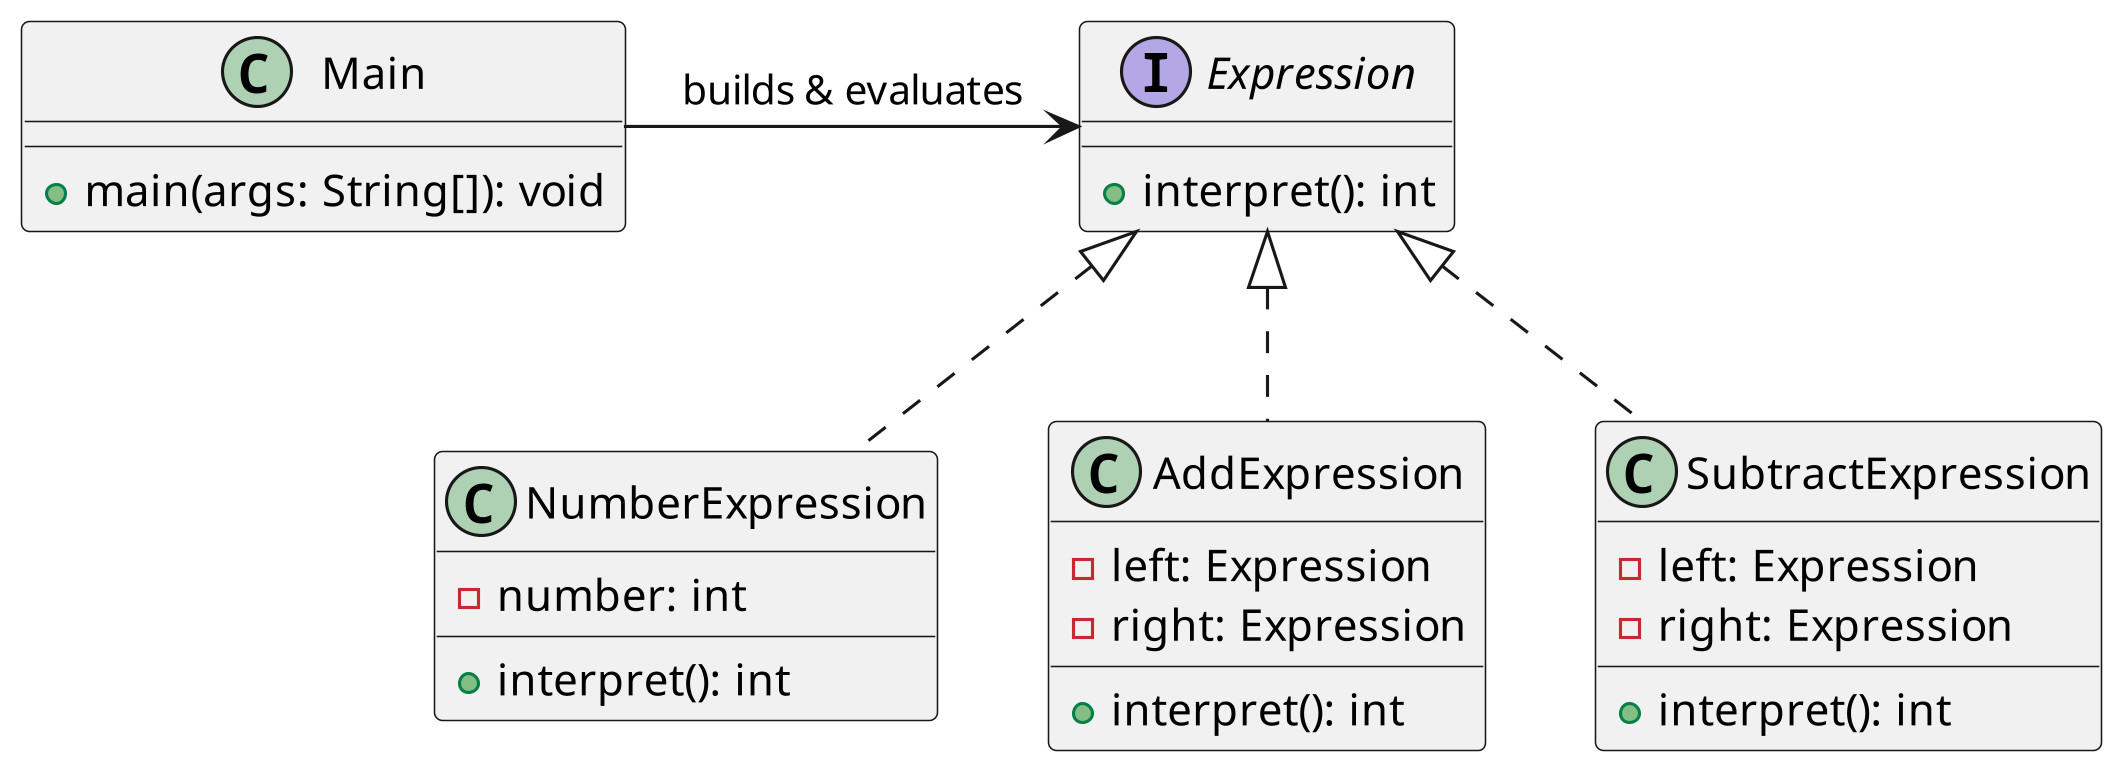
\includegraphics[width=\textwidth]{../figures/out/interpreter.png}
	\caption{Struktur Pola Interpreter}
	\label{fig:interpreter}
\end{figure}


Contoh berikut memperlihatkan penerapan pola \textit{Interpreter} untuk memproses ekspresi aritmatika sederhana dengan operasi penjumlahan dan pengurangan (Gambar \ref{fig:interpreter}).

\begin{lstlisting}[style=JavaStyle, caption={Antarmuka Ekspresi}, label={lst:interpreter-interface}]
	public interface Expression {
		int interpret();
	}
\end{lstlisting}

\begin{lstlisting}[style=JavaStyle, caption={Ekspresi Konstanta (Leaf)}, label={lst:interpreter-number}]
	public class NumberExpression implements Expression {
		private int number;
		
		public NumberExpression(int number) {
			this.number = number;
		}
		
		@Override
		public int interpret() {
			return number;
		}
	}
\end{lstlisting}

\begin{lstlisting}[style=JavaStyle, caption={Ekspresi Penjumlahan}, label={lst:interpreter-plus}]
	public class AddExpression implements Expression {
		private Expression left;
		private Expression right;
		
		public AddExpression(Expression left, Expression right) {
			this.left = left;
			this.right = right;
		}
		
		@Override
		public int interpret() {
			return left.interpret() + right.interpret();
		}
	}
\end{lstlisting}

\begin{lstlisting}[style=JavaStyle, caption={Ekspresi Pengurangan}, label={lst:interpreter-minus}]
	public class SubtractExpression implements Expression {
		private Expression left;
		private Expression right;
		
		public SubtractExpression(Expression left, Expression right) {
			this.left = left;
			this.right = right;
		}
		
		@Override
		public int interpret() {
			return left.interpret() - right.interpret();
		}
	}
\end{lstlisting}

\begin{lstlisting}[style=JavaStyle, caption={Client: Evaluasi Ekspresi}, label={lst:interpreter-main}]
	public class Main {
		public static void main(String[] args) {
			Expression expr = new AddExpression(
			new NumberExpression(10),
			new SubtractExpression(
			new NumberExpression(5),
			new NumberExpression(2)
			)
			);
			
			System.out.println("Result: " + expr.interpret()); // Output: 13
		}
	}
\end{lstlisting}

Pada contoh di atas:
\begin{itemize}
	\item \texttt{Expression} adalah antarmuka dasar untuk semua jenis ekspresi.
	\item \texttt{NumberExpression} adalah ekspresi terminal (leaf) yang hanya menyimpan nilai numerik.
	\item \texttt{AddExpression} dan \texttt{SubtractExpression} adalah ekspresi non-terminal (komposit) yang membentuk ekspresi kompleks dari dua ekspresi lainnya.
	\item Evaluasi dilakukan dengan memanggil \texttt{interpret()} secara rekursif, menyusun hasil dari anak-anak ekspresi.
\end{itemize}

Pola ini dapat dikembangkan lebih lanjut untuk mendukung ekspresi logika, ekspresi variabel dengan konteks (\texttt{Map<String, Integer> context}), atau ekspresi boolean, tergantung pada kebutuhan bahasa domain yang ingin diinterpretasi. Pendekatan ini cocok untuk membangun evaluator DSL (Domain-Specific Language) kecil dan sistem konfigurasi ekspresif.


\section{Observer}

\subsection{Tujuan dan Konteks Penggunaan}

Pola \textit{Observer} merupakan salah satu pola perilaku yang dirancang untuk mendefinisikan relasi satu-ke-banyak antara objek, di mana ketika satu objek (disebut \texttt{Subject}) mengalami perubahan status, seluruh objek lain yang bergantung padanya (disebut \texttt{Observer}) akan diberi notifikasi secara otomatis. Tujuan utama dari pola ini adalah untuk memastikan konsistensi antar objek tanpa menciptakan keterikatan (coupling) secara langsung di antara mereka.

Dengan menggunakan pola \textit{Observer}, sistem menjadi lebih fleksibel dalam menangani skenario di mana satu perubahan harus disebarkan ke banyak bagian lain dalam sistem. Pola ini mendukung prinsip \textit{Loose Coupling} karena \texttt{Subject} tidak perlu mengetahui secara spesifik siapa saja observer-nya, cukup dengan mengelola daftar observer dan memanggil metode \texttt{update()} ketika terjadi perubahan.

Pola ini sangat berguna dalam situasi di mana:
\begin{itemize}
	\item Objek data sering berubah dan perlu memberi tahu banyak bagian sistem (misalnya, tampilan antarmuka) setiap kali terjadi perubahan.
	\item Sistem membutuhkan arsitektur berbasis event, di mana komponen dapat bereaksi terhadap perubahan tanpa saling bergantung secara langsung.
	\item Perlu ada pemisahan antara data dan representasi (misalnya dalam pola \textit{Model-View-Controller}).
\end{itemize}

Komponen utama dalam pola \textit{Observer} meliputi:
\begin{enumerate}
	\item \textbf{Subject (Observable)}: Objek inti yang menyimpan data atau status. Menyediakan antarmuka untuk menambah, menghapus, dan memberi notifikasi kepada observer.
	\item \textbf{Observer}: Objek-objek yang ingin diberi tahu saat \texttt{Subject} berubah. Menerapkan antarmuka tertentu dengan metode seperti \texttt{update()}.
	\item \textbf{ConcreteSubject dan ConcreteObserver}: Implementasi spesifik dari subject dan observer yang berisi logika bisnis masing-masing.
\end{enumerate}

Pola \textit{Observer} secara luas digunakan dalam berbagai sistem, termasuk:
\begin{itemize}
	\item Aplikasi GUI (misalnya, Swing atau JavaFX), di mana perubahan pada model data perlu memperbarui elemen UI secara otomatis.
	\item Sistem event handling atau sistem messaging.
	\item Arsitektur publish-subscribe, di mana klien dapat mendaftar pada topik tertentu dan menerima notifikasi saat event terjadi.
\end{itemize}

Dengan menerapkan pola \textit{Observer}, sistem menjadi lebih modular, dapat dikembangkan secara independen, dan mudah diadaptasi untuk berbagai kebutuhan reaktivitas antar komponen.

\subsection{Contoh Kasus Penggunaan}

Pola \textit{Observer} banyak digunakan dalam sistem perangkat lunak yang membutuhkan mekanisme notifikasi otomatis ketika terjadi perubahan status pada suatu objek. Berikut adalah beberapa contoh kasus penggunaan nyata di berbagai domain:

\textbf{1. Antarmuka Pengguna (User Interface):}  
Dalam aplikasi desktop atau mobile, pola \textit{Observer} digunakan untuk memastikan bahwa komponen tampilan (View) selalu konsisten dengan model data. Ketika data diubah, tampilan yang terdaftar sebagai observer akan diperbarui secara otomatis. Misalnya, dalam arsitektur Model-View-Controller (MVC), komponen View menjadi observer terhadap perubahan dalam Model.

\textbf{2. Sistem Event Handling:}  
Sistem seperti Java AWT/Swing, atau event bus pada framework modern, mengandalkan pola ini untuk mengatur komunikasi antara objek. Misalnya, tombol (\texttt{Button}) sebagai \texttt{Subject} akan memberi tahu listener (\texttt{Observer}) ketika diklik. Dengan demikian, berbagai komponen dapat merespons aksi pengguna secara dinamis tanpa saling bergantung.

\textbf{3. Sinkronisasi Data Antarkomponen:}  
Dalam aplikasi spreadsheet atau grafis, ketika satu sel atau objek diubah, seluruh komponen terkait (misalnya grafik atau hasil perhitungan lain) perlu diperbarui. Pola \textit{Observer} memungkinkan penyebaran perubahan ini secara otomatis tanpa menghubungkan komponen secara langsung.

\textbf{4. Sistem Notifikasi:}  
Aplikasi berita, media sosial, dan platform komunikasi menggunakan pola ini untuk memberi tahu pengguna saat ada konten baru. Misalnya, pengguna yang mengikuti topik atau akun tertentu akan menerima notifikasi saat topik tersebut diperbarui. Di balik layar, topik berperan sebagai \texttt{Subject}, dan pengguna sebagai \texttt{Observer}.

\textbf{5. Sistem Monitoring dan Logging:}  
Dalam sistem server atau aplikasi terdistribusi, modul pemantauan dapat bertindak sebagai observer terhadap status komponen sistem. Jika suatu komponen gagal, observer akan mencatat log, mengirim email, atau memicu alur pemulihan secara otomatis.

\textbf{6. Pasar Keuangan dan Data Feed:}  
Aplikasi perdagangan saham atau crypto biasanya membutuhkan data pasar real-time. Modul antarmuka pasar bertindak sebagai \texttt{Subject}, dan berbagai modul seperti tampilan harga, strategi trading, dan notifikasi akan mendaftar sebagai observer untuk menerima update harga terbaru.

Pola \textit{Observer} sangat bermanfaat ketika dibutuhkan penyebaran perubahan ke banyak bagian sistem secara otomatis, tanpa mengikat implementasi secara langsung. Pendekatan ini meningkatkan skalabilitas dan keterpisahan logika antar komponen.

\subsection{Kelebihan dan Kekurangan}

Pola \textit{Observer} menawarkan mekanisme yang efektif untuk mengatur komunikasi satu-ke-banyak antara objek-objek dalam sistem. Namun, seperti semua pola desain, penerapannya memiliki kelebihan dan kekurangan yang perlu dipertimbangkan secara cermat sesuai konteks penggunaannya.

\textbf{Kelebihan:}
\begin{itemize}
	\item \textbf{Dekopling antara Subject dan Observer:} Subjek tidak perlu mengetahui detail implementasi observer; hanya perlu tahu bahwa mereka mengikuti antarmuka tertentu. Ini meningkatkan modularitas dan fleksibilitas sistem.
	
	\item \textbf{Mendukung mekanisme notifikasi otomatis:} Perubahan pada satu objek secara otomatis disebarkan ke semua observer, sehingga data dan tampilan selalu sinkron tanpa perlu intervensi manual.
	
	\item \textbf{Mudah diperluas:} Observer baru dapat ditambahkan kapan saja tanpa memodifikasi kode dari subjek. Hal ini sejalan dengan prinsip Open/Closed.
	
	\item \textbf{Meningkatkan reaktivitas sistem:} Cocok untuk sistem real-time dan event-driven di mana banyak bagian perlu merespons satu peristiwa yang sama.
	
	\item \textbf{Penerapan yang luas dan terstandarisasi:} Telah didukung secara native di banyak bahasa dan framework, seperti Java (\texttt{Observer/Observable}) dan C\# (event dan delegate).
\end{itemize}

\textbf{Kekurangan:}
\begin{itemize}
	\item \textbf{Sulit ditelusuri dan diuji:} Karena efek samping dari notifikasi tersebar ke banyak observer, jejak eksekusi bisa menjadi kompleks dan sulit ditelusuri saat debugging.
	
	\item \textbf{Potensi masalah kinerja:} Jika jumlah observer sangat banyak atau logika update terlalu berat, notifikasi dapat menyebabkan penurunan performa.
	
	\item \textbf{Keterkaitan implisit:} Meskipun secara teknis terpisah, ada ketergantungan implisit antara subjek dan observer yang bisa menyebabkan dampak tak terduga jika tidak dikelola dengan baik.
	
	\item \textbf{Masalah memori (memory leaks):} Jika observer tidak dihapus secara eksplisit dari daftar observer subjek, maka objek bisa terus berada dalam memori (terutama dalam bahasa tanpa garbage collection otomatis terhadap referensi terdaftar).
	
	\item \textbf{Urutan notifikasi tidak terjamin:} Observer biasanya diberi tahu tanpa urutan yang pasti, yang bisa menjadi masalah jika ada ketergantungan antar observer dalam pengolahan data.
\end{itemize}

Secara keseluruhan, pola \textit{Observer} sangat berguna untuk membangun sistem yang reaktif, modular, dan mudah diperluas. Namun, harus digunakan dengan kehati-hatian dalam sistem besar dan kompleks untuk menghindari masalah skalabilitas dan pemelihar


\subsection{Implementasi dalam Java}

Implementasi pola \textit{Observer} dalam Java dapat dilakukan dengan dua pendekatan utama: menggunakan antarmuka buatan sendiri atau menggunakan API standar Java. Sejak Java 9, kelas bawaan \texttt{Observable} telah dinyatakan deprecated, sehingga pendekatan berbasis antarmuka lebih disarankan untuk fleksibilitas dan pemahaman konsep yang lebih dalam.


\begin{figure}[h]
	\centering
	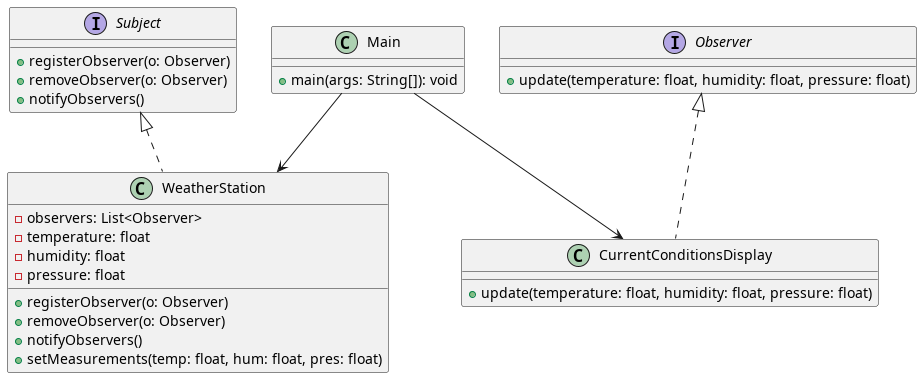
\includegraphics[width=\textwidth]{../figures/out/observer.png}
	\caption{Struktur Pola Observer}
	\label{fig:observer}
\end{figure}

Contoh berikut menunjukkan cara mengimplementasikan pola \textit{Observer} secara manual dengan mendefinisikan antarmuka \texttt{Observer} dan \texttt{Subject}, serta kelas \texttt{WeatherStation} sebagai subjek dan beberapa kelas \texttt{Display} sebagai observer (Gambar \ref{fig:observer}).

\begin{lstlisting}[style=JavaStyle, caption={Antarmuka Subject dan Observer}]
	public interface Observer {
		void update(float temperature, float humidity, float pressure);
	}
	
	public interface Subject {
		void registerObserver(Observer o);
		void removeObserver(Observer o);
		void notifyObservers();
	}
\end{lstlisting}

\begin{lstlisting}[style=JavaStyle, caption={Kelas WeatherStation sebagai Subject}]
	import java.util.*;
	
	public class WeatherStation implements Subject {
		private List<Observer> observers = new ArrayList<>();
		private float temperature, humidity, pressure;
		
		@Override
		public void registerObserver(Observer o) {
			observers.add(o);
		}
		
		@Override
		public void removeObserver(Observer o) {
			observers.remove(o);
		}
		
		@Override
		public void notifyObservers() {
			for (Observer o : observers) {
				o.update(temperature, humidity, pressure);
			}
		}
		
		public void setMeasurements(float temp, float hum, float pres) {
			this.temperature = temp;
			this.humidity = hum;
			this.pressure = pres;
			notifyObservers();
		}
	}
\end{lstlisting}

\begin{lstlisting}[style=JavaStyle, caption={Observer: CurrentConditionsDisplay}]
	public class CurrentConditionsDisplay implements Observer {
		@Override
		public void update(float temperature, float humidity, float pressure) {
			System.out.println("Current Conditions: " + temperature 
			+ " C, " + humidity + "% humidity, " + pressure + " hPa");
		}
	}
\end{lstlisting}

\begin{lstlisting}[style=JavaStyle, caption={Client: Main}]
	public class Main {
		public static void main(String[] args) {
			WeatherStation station = new WeatherStation();
			Observer display = new CurrentConditionsDisplay();
			
			station.registerObserver(display);
			station.setMeasurements(26.5f, 65f, 1012f);
		}
	}
\end{lstlisting}

Pada contoh di atas:
\begin{itemize}
	\item \texttt{WeatherStation} adalah kelas yang berperan sebagai \texttt{Subject} dan menyimpan daftar observer.
	\item \texttt{CurrentConditionsDisplay} adalah salah satu implementasi dari \texttt{Observer} yang bereaksi terhadap perubahan.
	\item Metode \texttt{setMeasurements()} mengubah nilai cuaca dan memberi tahu semua observer secara otomatis.
\end{itemize}

Pendekatan ini menunjukkan kekuatan pola \textit{Observer} dalam menciptakan sistem yang reaktif dan loosely-coupled, memungkinkan klien menambahkan atau menghapus observer tanpa mengubah kode subjek.

\section{Kesimpulan}
Pola \textit{Interpreter} menyediakan kerangka kerja untuk memproses ekspresi atau bahasa domain secara sistematis. Terakhir, \textit{Observer} mendukung arsitektur reaktif dan event-driven dengan menyebarkan notifikasi perubahan status secara otomatis ke banyak objek terkait.